% Using Free and Open Source Solutions in Geospatial Science Education
% This work by Vaclav Petras is licensed under
% a Creative Commons Attribution-ShareAlike 4.0 International License.

\documentclass[xcolor={dvipsnames,usenames},beamer,aspectratio=43]{beamer}
% ,handout,notes=show

\makeatletter
\def\beamer@framenotesbegin{% at beginning of slide
  \gdef\beamer@noteitems{}%
  \gdef\beamer@notes{{}}% used to be totally empty.
}
\makeatother

\usepackage{textcomp}
\usepackage[utf8]{inputenc}
\usepackage[american]{babel}
\usepackage{graphicx}
\usepackage{url}
\usepackage{amssymb}

\usepackage{alltt}

\usepackage{tikz}
\usetikzlibrary{arrows,shapes,spy,calc}

\tikzstyle{every picture}+=[remember picture]
\tikzstyle{na} = [baseline=-.5ex]

% don't count bacup slides
\newcommand{\backupbegin}{
   \newcounter{finalframe}
   \setcounter{finalframe}{\value{framenumber}}
}
\newcommand{\backupend}{
   \setcounter{framenumber}{\value{finalframe}}
}

% frames have to be fragile
\newif\ifnotes
% \input{tmpnotessettings}
% \notestrue


\ifnotes
\setbeamertemplate{note page}[plain]
% \setbeamertemplate{note page}[compress]
\setbeamerfont{note page}{size=\large}
% \setbeameroption{show only notes}
\setbeameroption{show notes}
\usepackage{pgfpages}
\pgfpagesuselayout{2 on 1}[a4paper,border shrink=5mm]%
\else
%\setbeameroption{hide notes}
\fi
%\notesfalse

\usepackage[absolute,overlay]{textpos}

\usepackage{listings}


% \usetheme{Warsaw}
\usetheme{Madrid}
% \usetheme{Frankfurt}
% \useoutertheme{infolines}
\usecolortheme[named=MidnightBlue]{structure}
% \usecolortheme[named=PineGreen]{structure}
\setbeamertemplate{navigation symbols}{}

\setbeamertemplate{itemize items}[default]
\setbeamertemplate{enumerate items}[default]
% \useinnertheme{rectangles}
\setbeamertemplate{blocks}[default]


%%%%%%%%%%%%%%%%%%%%%%%%%%%%%%%%%%%%%%%%%%%%%%%%%%%%%%%%%%%%%%%%%%%%
%%%%%%%%%%%%%%%%%%%%%%%%%%%%%%%%%%%%%%%%%%%%%%%%%%%%%%%%%%%%%%%%%%%%

% \newcommand{\n}[1]{$^{\color{gray}{\mbox{\tiny#1}}}$}
\newcommand{\n}[1]{$^{\textcolor{gray}{\mbox{\tiny #1}}}$}

%%%%%%%%%%%%%%%%%%%%%%%%%%%%%%%%%%%%%%%%%%%%%%%%%%%%%%%%%%%%%%%%%%%%%%%%%%%%%%%
\newcommand{\gmodule}[1]{\href{http://grass.osgeo.org/grass71/manuals/#1.html}{\emph{#1}}}
\newcommand{\amodule}[1]{\href{http://grass.osgeo.org/grass70/manuals/addons/#1.html}{\emph{#1}}}
\newcommand{\module}[1]{\emph{#1}}
\newcommand{\grasslink}{\href{http://grass.osgeo.org/}{GRASS GIS}}

%%%%%%%%%%%%%%%%%%%%%%%%%%%%%%%%%%%%%%%%%%%%%%%%%%%%%%%%%%%%%%%%%%%%
%%%%%%%%%%%%%%%%%%%%%%%%%%%%%%%%%%%%%%%%%%%%%%%%%%%%%%%%%%%%%%%%%%%%

\title{GRASS GIS loves lidar}
\subtitle{FOSS4G NA 2016}
%\pdforstring{}{}

\author[Vaclav Petras]
{Vaclav Petras (Vashek)\\%\n{1,2}\\
{
\scriptsize
Anna Petrasova, %\n{3},
%\mbox{
Helena Mitasova%\n{1,2}
%}
}
}

\institute[NC State University]
{%
Center for Geospatial Analytics
% \tiny
%\n{1}NCSU Department of Marine, Earth and Atmospheric Sciences \\
%\n{2}NCSU Center for Geospatial Analytics \\
%\n{3}U.S. Fish and Wildlife Service

\bigskip

\includegraphics[width=0.3\textwidth]{logos/ncstate}
}

\date{May 5, 2016}

\setbeamercovered{transparent}

\hypersetup{%
 pdfauthor={Vaclav Petras},%
 pdfsubject={GRASS GIS and point clouds talk at FOSS4G NA 2016},%
 pdfkeywords={UAV} {UAS} {point clouds} {lidar}
   {v.in.lidar} {r.in.lidar} {v.decimate} {r.in.kinect} {v.out.lidar} {libLAS} {PDAL} {PCL}
   {geospatial modeling} {GRASS GIS}
   {free software} {open source} {open science}
}

\usepackage{tipa}
\newcommand{\pron}[2]{#1 [#2]}


%%%%%%%%%%%%%%%%%%%%%%%%%%%%%%%%%%%%%%%%%%%%%%%%%%%%%%%%%%%%%%%%%%%%
% when images are placed in these directories, we don't have to specify the directory
% just the filename
\graphicspath{{img/}{figures/}{images/}}


%%%%%%%%%%%%%%%%%%%%%%%%%%%%%%%%%%%%%%%%%%%%%%%%%%%%%%%%%%%%%%%%%%%%
%%%%%%%%%%%%%%%%%%%%%%%%%%%%%%%%%%%%%%%%%%%%%%%%%%%%%%%%%%%%%%%%%%%%
%%%%%%%%%%%%%%%%%%%%%%%%%%%%%%%%%%%%%%%%%%%%%%%%%%%%%%%%%%%%%%%%%%%%
%%%%%%%%%%%%%%%%%%%%%%%%%%%%%%%%%%%%%%%%%%%%%%%%%%%%%%%%%%%%%%%%%%%%
\begin{document}

\newcommand{\logowidth}{1.0em}
\newcommand{\logospace}{\hspace{0.2em}}
\newcommand{\includecclogo}[1]{\includegraphics[width=\logowidth]{./images/logos/#1}}

%%%%%%%%%%%%%%%%%%%%%%%%%%%%%%%%%%%%%%%%%%%%%%%%%%%%%%%%%%%%%%%%%%%%
\frame{
\titlepage
\begin{center}
\vspace{-3ex}
\href{http://creativecommons.org/licenses/by-sa/4.0/}{
\includecclogo{cc}
\logospace
\includecclogo{by}
\logospace
\includecclogo{sa}
}
\\
\footnotesize
available at\\
\href{http://wenzeslaus.github.io/grass-lidar-talks/}{\texttt{wenzeslaus.github.io/grass-lidar-talks}}
\end{center}
}


%%%%%%%%%%%%%%%%%%%%%%%%%%%%%%%%%%%%%%%%%%%%%%%%%%%%%%%%%%%%%%%%%%%%%
\begin{frame}{GRASS GIS}

\begin{columns}
\begin{column}{0.6\textwidth}

\begin{itemize}
  \item all in one
  \begin{itemize}
   \item hydrology modeling, image segmentation, point clustering, \ldots
  \end{itemize}
  \item from small laptops to supercomputers
  \begin{itemize}
   \item Raspberry Pi, Windows, Mac, GNU/Linux, GNU/Hurd, FreeBSD, IBM~AIX
  \end{itemize}
  \item learn now, use forever
  \begin{itemize}
    \item over 30 years of development and interface refinement
  \end{itemize}
  \item probably used more than you think
  \begin{itemize}
    \item similarly to C/C++ is often not mentioned but is somewhere in there
  \end{itemize}
\end{itemize}

\end{column}
\begin{column}{0.3\textwidth}

\begin{center}
  
\includegraphics[width=\textwidth]{logos/grass_gis}
\end{center}

\textcolor{gray}{
\footnotesize
latest release 7.0.4 Sunday, May~1,~2016
}

\end{column}
\end{columns}

\end{frame}


%%%%%%%%%%%%%%%%%%%%%%%%%%%%%%%%%%%%%%%%%%%%%%%%%%%%%%%%%%%%%%%%%%%%%
\begin{frame}{CLI}

\begin{center}
  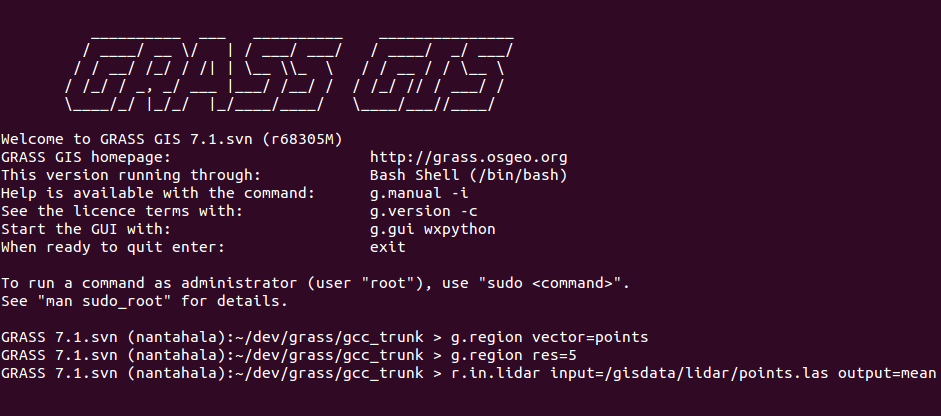
\includegraphics[width=0.9\textwidth]{grass/grass_cli}
\end{center}

\end{frame}


%%%%%%%%%%%%%%%%%%%%%%%%%%%%%%%%%%%%%%%%%%%%%%%%%%%%%%%%%%%%%%%%%%%%%
\begin{frame}{GUI}

\begin{center}
  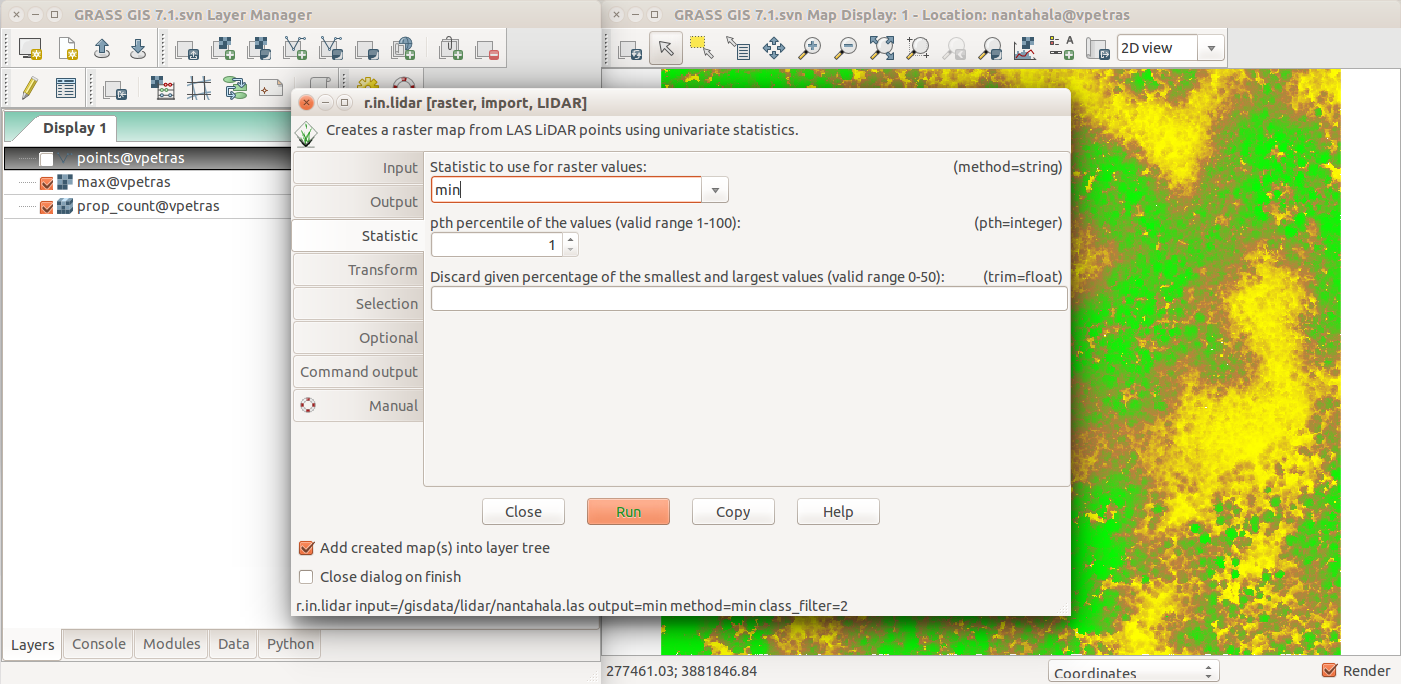
\includegraphics[width=0.9\textwidth]{grass/r_in_lidar_gui}
\end{center}

\end{frame}


%%%%%%%%%%%%%%%%%%%%%%%%%%%%%%%%%%%%%%%%%%%%%%%%%%%%%%%%%%%%%%%%%%%%%
\begin{frame}{Python}

\begin{center}
  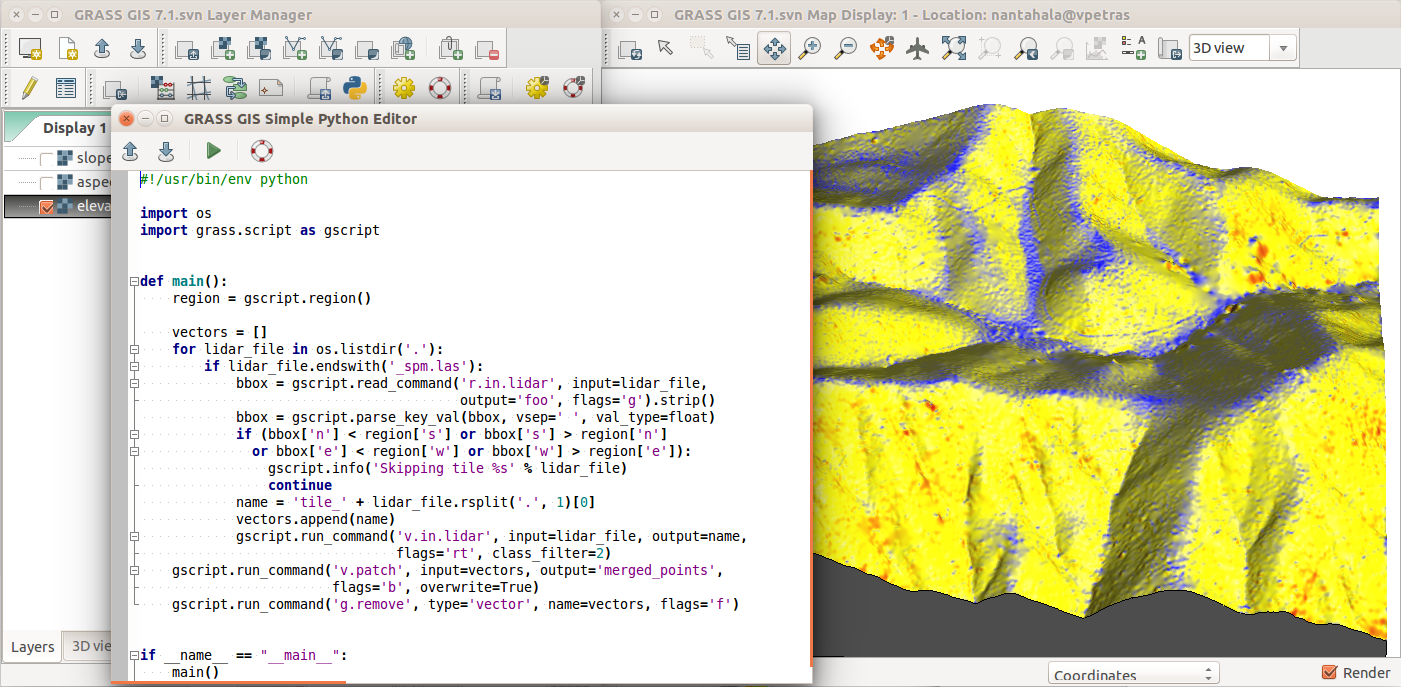
\includegraphics[width=0.9\textwidth]{grass/grass_pyedit}
\end{center}

\end{frame}


%%%%%%%%%%%%%%%%%%%%%%%%%%%%%%%%%%%%%%%%%%%%%%%%%%%%%%%%%%%%%%%%%%%%%
\begin{frame}{Python versus CLI}

\definecolor{mod}{RGB}{7,96,143}
\definecolor{opt}{RGB}{239,84,18}
\definecolor{flg}{RGB}{239,84,18}
\definecolor{txt}{RGB}{45,146,45}
\definecolor{bash}{RGB}{200,200,200}
\definecolor{import}{RGB}{200,200,200}

\Large

Documentation, Command Line (Shell, Bash, cmd.exe):

\LARGE

\begin{alltt}
\textcolor{mod}{r.in.lidar} \textcolor{opt}{input}=\textcolor{txt}{points.las} \textcolor{bash}{\char`\\}
\\%
\newlength{\shindent}
\settowidth{\shindent}{r.in.lidar~}
\rule{\shindent}{0pt}%
\textcolor{opt}{output}=\textcolor{txt}{elevation} -\textcolor{flg}{e}
\end{alltt}

\Large

Python:

% \char`_ is to get same underscore as in \verb

\LARGE

\begin{alltt}
\textcolor{import}{from grass.script import run\char`_command}
\\
run\char`_command('\textcolor{mod}{r.in.lidar}',
%
\newlength{\pyindent}%
\settowidth{\pyindent}{run\_command(}%
\\%
\rule{\pyindent}{0pt}\,%
\textcolor{opt}{input}="\textcolor{txt}{points.las}",
\\%
\rule{\pyindent}{0pt}\,%
\textcolor{opt}{output}="\textcolor{txt}{elevation}",
\\%
\rule{\pyindent}{0pt}\,%
flags='\textcolor{flg}{e}')
\end{alltt}

\end{frame}


%%%%%%%%%%%%%%%%%%%%%%%%%%%%%%%%%%%%%%%%%%%%%%%%%%%%%%%%%%%%%%%%%%%%%
\begin{frame}{Module GUI}

\begin{center}
  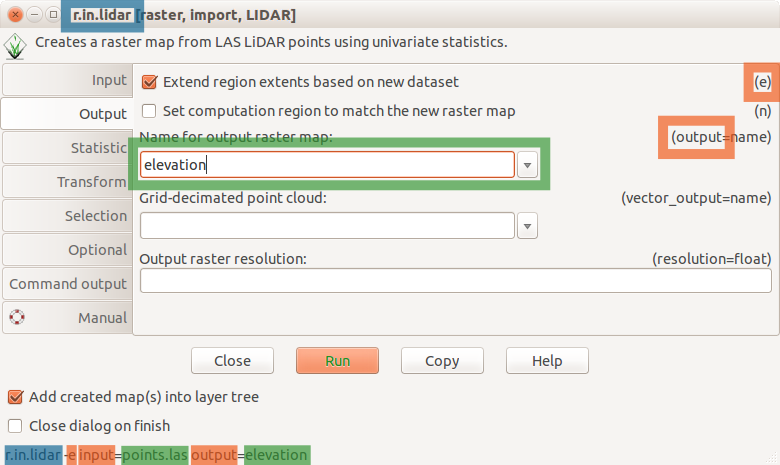
\includegraphics[width=0.75\textwidth]{grass/r_in_lidar_dialog}
\end{center}

\end{frame}


%%%%%%%%%%%%%%%%%%%%%%%%%%%%%%%%%%%%%%%%%%%%%%%%%%%%%%%%%%%%%%%%%%%%%
\begin{frame}{Graphical Modeler}

\begin{center}
  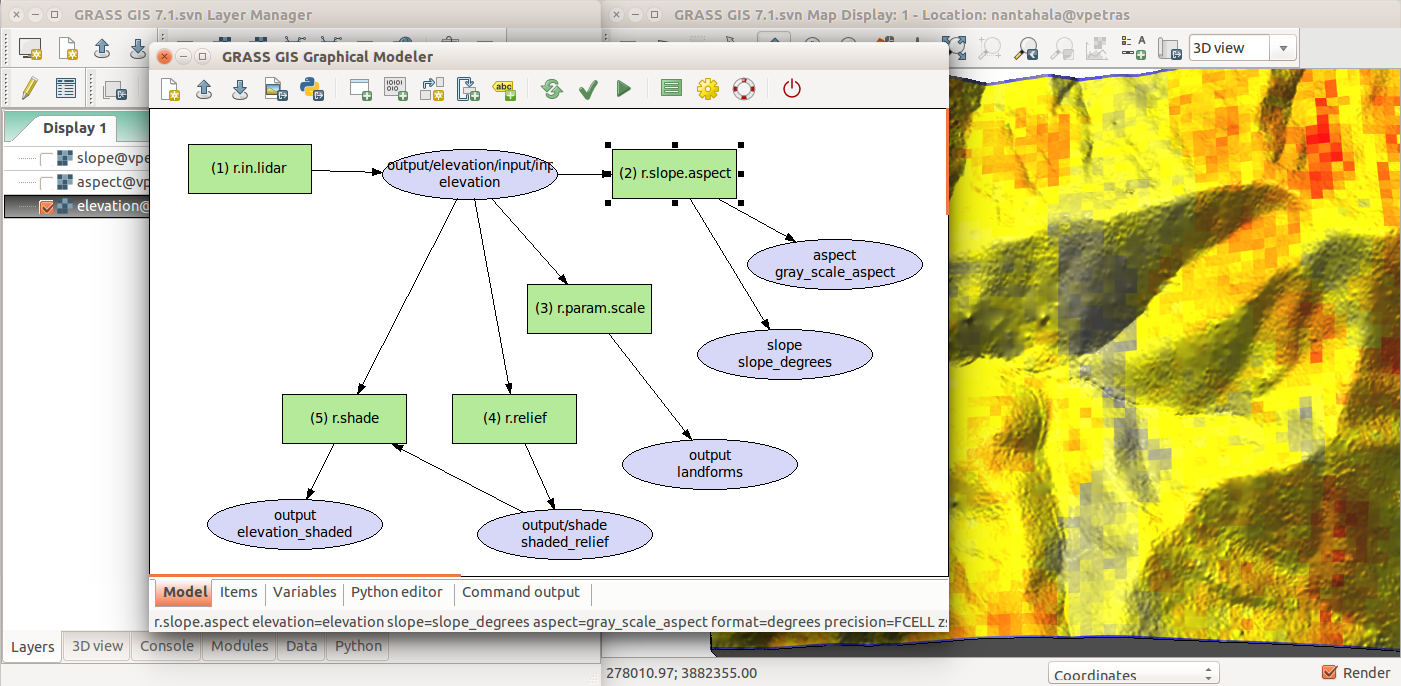
\includegraphics[width=0.9\textwidth]{grass/modeler}
\end{center}

\end{frame}


%%%%%%%%%%%%%%%%%%%%%%%%%%%%%%%%%%%%%%%%%%%%%%%%%%%%%%%%%%%%%%%%%%%%%
\begin{frame}{Points}

\begin{columns}
\begin{column}{0.3\textwidth}

\begin{itemize}
  \item collected by lidar
  \item generated by Structure from Motion (SfM) from UAV imagery
  \item a lot of points
\end{itemize}

\end{column}
\begin{column}{0.65\textwidth}

\begin{center}
  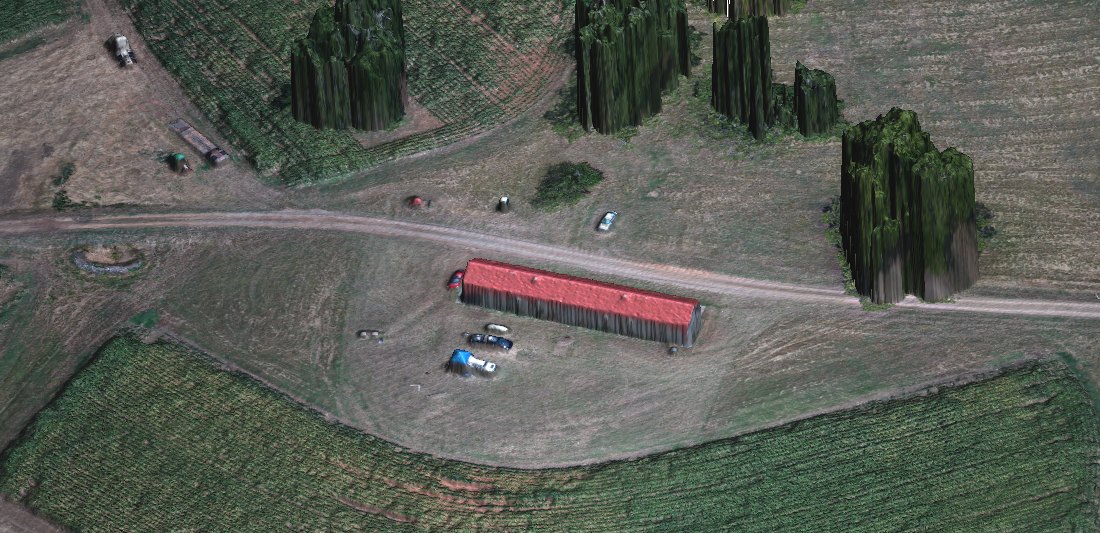
\includegraphics[width=\textwidth]{agisoft_detail}
  \\
  \tiny
  \textcolor{gray}{surface interpolated from points and visualized in GRASS GIS}
\end{center}

\end{column}
\end{columns}

\end{frame}


%%%%%%%%%%%%%%%%%%%%%%%%%%%%%%%%%%%%%%%%%%%%%%%%%%%%%%%%%%%%%%%%%%%%%
\begin{frame}{Workflow overview}

\includegraphics[width=\textwidth]%
    {grass/workflow}

\end{frame}


%%%%%%%%%%%%%%%%%%%%%%%%%%%%%%%%%%%%%%%%%%%%%%%%%%%%%%%%%%%%%%%%%%%%%
\begin{frame}{Surface interpolation}

\begin{columns}
\begin{column}{0.5\textwidth}

\begin{itemize}
  \item \gmodule{v.surf.idw}
  \begin{itemize}
    \item Inverse Distance squared Weighting
  \end{itemize}
  \item \gmodule{v.surf.bspline}
  \begin{itemize}
    \item Bicubic or bilinear Spline interpolation with Tykhonov regularization
  \end{itemize}
  \item \gmodule{v.surf.rst}
  \begin{itemize}
    \item Regularized Spline with Tension
    \item \gmodule{v.surf.rst.mp} (experimental)
    \begin{itemize}
      \item 2 millions of points in 11~minutes
    \end{itemize}
  \end{itemize}
\end{itemize}

\end{column}
\begin{column}{0.4\textwidth}

\begin{center}
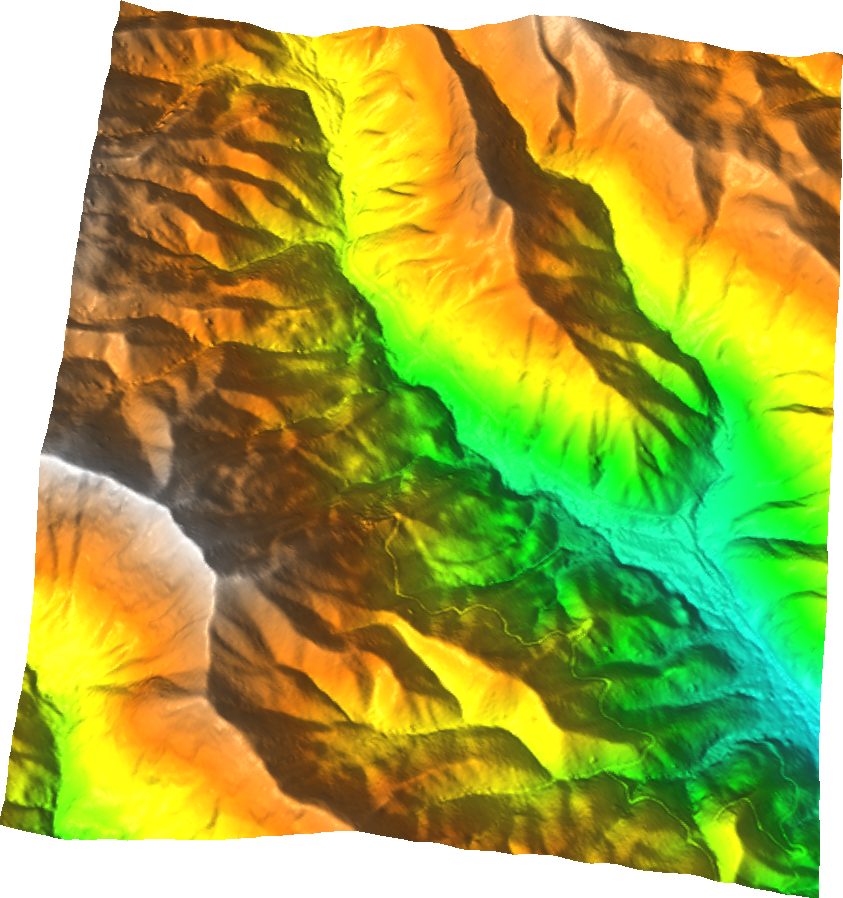
\includegraphics[width=\textwidth]{features/surface}
\end{center}

\end{column}
\end{columns}

\end{frame}


%%%%%%%%%%%%%%%%%%%%%%%%%%%%%%%%%%%%%%%%%%%%%%%%%%%%%%%%%%%%%%%%%%%%%
\begin{frame}{Import and decimation}

\begin{columns}
\begin{column}{0.58\textwidth}

\begin{itemize}
  \item \gmodule{v.in.lidar}
  \begin{itemize}
   \item libLAS
   \item LAS/LAZ to GRASS GIS native vector
    \item data stored in GRASS GIS database
  \end{itemize}
  \item decimation~$\approx$~thinning~$\approx$~sampling
  \begin{itemize}
    \item count-based decimation (skips points)
    \item grid-based experimental, others needed?  % TODO: grid-based also through r.in.lidar
    \item fast count-based as good as more advanced decimations
  \end{itemize}
\end{itemize}

\end{column}
\begin{column}{0.22\textwidth}

% TODO: UAV image

\begin{center}
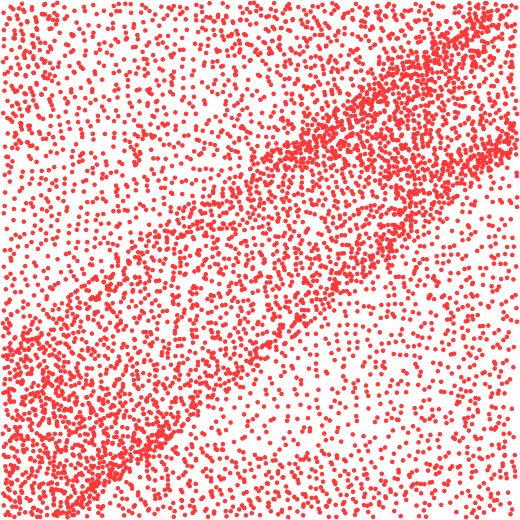
\includegraphics[width=\textwidth]{features/full}

\smallskip

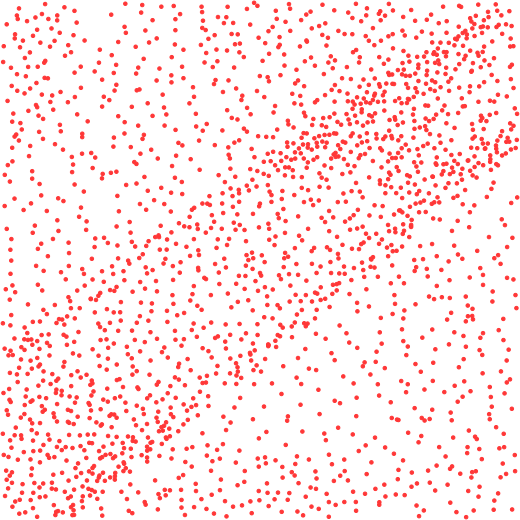
\includegraphics[width=\textwidth]{features/preserve}

\end{center}

\end{column}
\end{columns}

\end{frame}

%%%%%%%%%%%%%%%%%%%%%%%%%%%%%%%%%%%%%%%%%%%%%%%%%%%%%%%%%%%%%%%%%%%%%
\begin{frame}{GRASS vector model and format}

\begin{columns}
\begin{column}{0.45\textwidth}

\begin{itemize}
  \item topology and index
  \begin{itemize}
    \item can be disabled (\textit{-b} flag)
  \end{itemize}
  \item attributes in a database
  \begin{itemize}
    \item SQLite, PostgreSQL, \ldots
    \item can be disabled (\textit{-t} flag)
  \end{itemize}
  \item each feature can have any number of categories/classes%
  \begin{itemize}
    \item without attribute table
  \end{itemize}
\end{itemize}

\end{column}
\begin{column}{0.5\textwidth}

\begin{center}
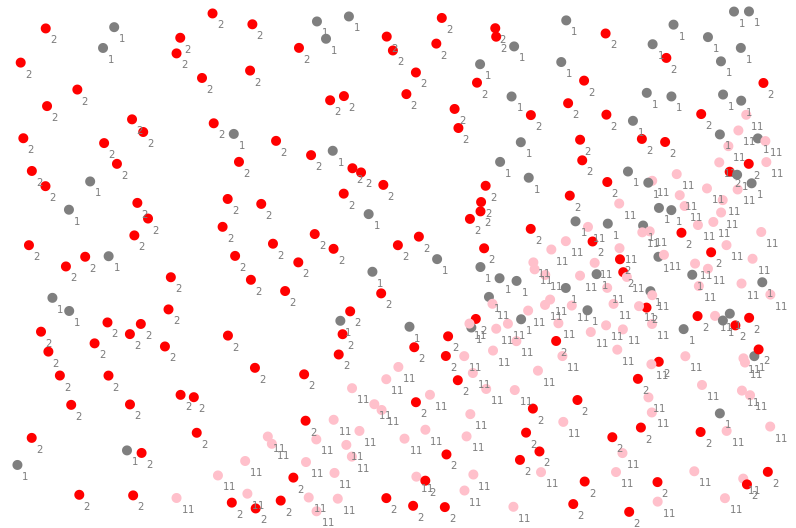
\includegraphics[width=\textwidth]{features/class_as_cat}
\end{center}

\end{column}
\end{columns}

\end{frame}

%%%%%%%%%%%%%%%%%%%%%%%%%%%%%%%%%%%%%%%%%%%%%%%%%%%%%%%%%%%%%%%%%%%%%
\begin{frame}{Linked external data}

\begin{columns}
\begin{column}{0.45\textwidth}

\begin{itemize}
  \item \gmodule{r.external}
  \begin{itemize}
    \item raster data (GDAL)
    \item \gmodule{r.external.out} for newly created data
  \end{itemize}
  \item \gmodule{v.external}
  \begin{itemize}
    \item vector data
    \begin{itemize}
      \item GDAL/OGR
      \item PostGIS including topology
    \end{itemize}
    \item \gmodule{v.external.out} for newly created data
    \item alternative: @OGR
      \\\tiny\texttt{v.info map=.../directory@OGR layer=file}
  \end{itemize}
\end{itemize}

\end{column}
\begin{column}{0.5\textwidth}

\begin{center}
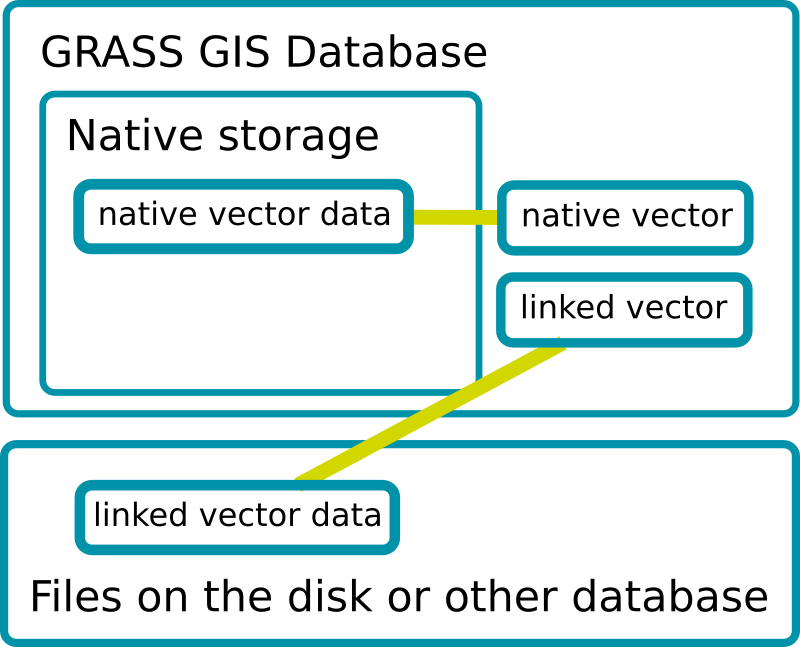
\includegraphics[width=\textwidth]{features/external_data}
\end{center}

\end{column}
\end{columns}

\begin{itemize}
  \item missing: libLAS/PDAL backend
  \begin{itemize}
    \item intermediate C API needed in PDAL or GRASS GIS
  \end{itemize}
\end{itemize}

\end{frame}

%%%%%%%%%%%%%%%%%%%%%%%%%%%%%%%%%%%%%%%%%%%%%%%%%%%%%%%%%%%%%%%%%%%%%
\begin{frame}{Current state of integration with PDAL}

\begin{columns}
\begin{column}{0.5\textwidth}

\begin{block}{PDAL}
 \begin{itemize}
  \item Point Data Abstraction Library
  \item format conversions
  \item processing, filtering
 \end{itemize}
\end{block}

\begin{block}{Experimental integration}
 \begin{itemize}
  \item \module{v.in.pdal}
  \begin{itemize}
    \item next: \module{r.in.pdal}, \module{r3.in.pdal}
  \end{itemize}
  \item runs PDAL filters during import
  \begin{itemize}
    \item filters are followed by GRASS processing
  \end{itemize}
 \end{itemize}
\end{block}

\end{column}
\begin{column}{0.25\textwidth}

\begin{center}
  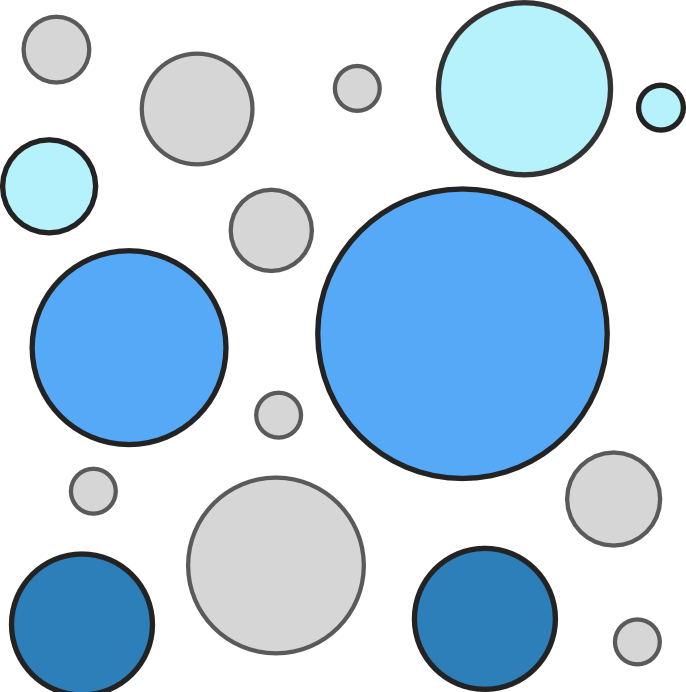
\includegraphics[width=\textwidth]{logos/pdal_bubbles}\\
  
\includegraphics[width=\textwidth]{logos/pdal_text}
\end{center}

\end{column}
\end{columns}

\end{frame}


%%%%%%%%%%%%%%%%%%%%%%%%%%%%%%%%%%%%%%%%%%%%%%%%%%%%%%%%%%%%%%%%%%%%%
\begin{frame}{Binning points to raster}

\begin{columns}
\begin{column}{0.4\textwidth}

 \begin{itemize}
  \item \gmodule{r.in.lidar}
  \item import and analysis
  \item statistics of point counts, height and intensity
  \begin{itemize}
    \item n, min, max, sum
    \item mean, range, skewness, \ldots
  \end{itemize}
\end{itemize}

\end{column}
\begin{column}{0.45\textwidth}

\begin{center}
  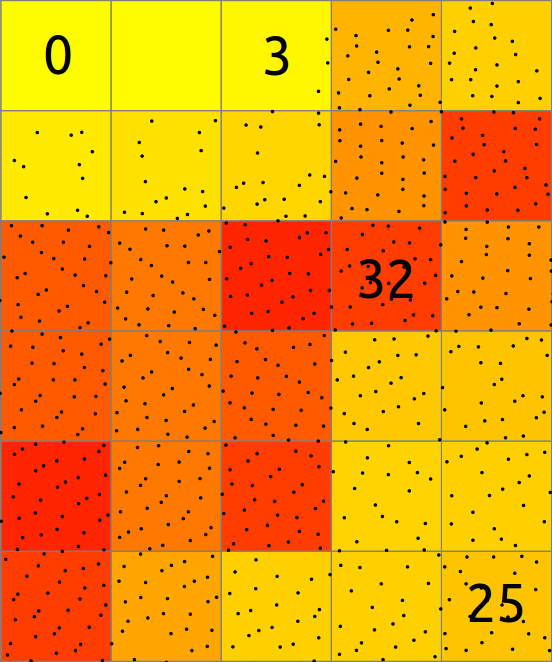
\includegraphics[width=0.75\textwidth]{features/binning_count}
\end{center}

\end{column}
\end{columns}

\end{frame}


%%%%%%%%%%%%%%%%%%%%%%%%%%%%%%%%%%%%%%%%%%%%%%%%%%%%%%%%%%%%%%%%%%%%%
\begin{frame}{Read multiple tiles as one}

\begin{columns}
\begin{column}{0.45\textwidth}

 \begin{itemize}
  \item \gmodule{r.in.lidar}, option \textit{file}
  %\begin{itemize}
    \begin{itemize}
    \item read multiple tiles as one
    \item no merging
    \end{itemize}
  %\end{itemize}
\end{itemize}

\textcolor{gray}{
\begin{center}
\tiny
0.5 billion points in 90 files in minutes
\end{center}
}

\end{column}
\begin{column}{0.54\textwidth}

\begin{center}
  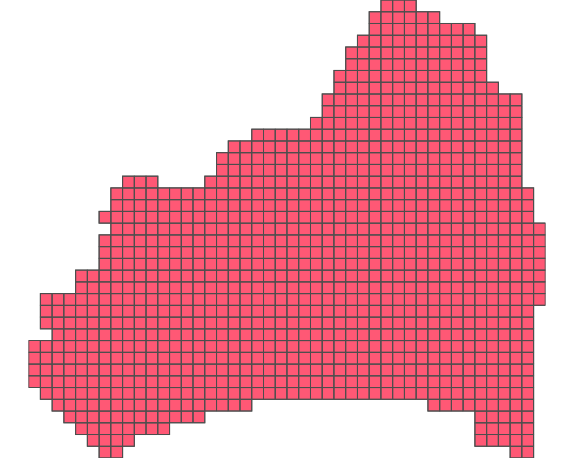
\includegraphics[width=\textwidth]{features/tiles}
\end{center}

\end{column}
\end{columns}

\end{frame}

%%%%%%%%%%%%%%%%%%%%%%%%%%%%%%%%%%%%%%%%%%%%%%%%%%%%%%%%%%%%%%%%%%%%%
\begin{frame}{Filtering points}

\begin{columns}
\begin{column}{0.45\textwidth}

 \begin{itemize}
  \item filter points by
  \begin{itemize}
    \item range of Z
    \item return
    \item class
    \item \ldots
  \end{itemize}
  \item at the time of binning with \gmodule{r.in.lidar}
    \begin{itemize}
    \item minimal additional cost
    \end{itemize}
\end{itemize}

\end{column}
\begin{column}{0.53\textwidth}

\begin{center}
  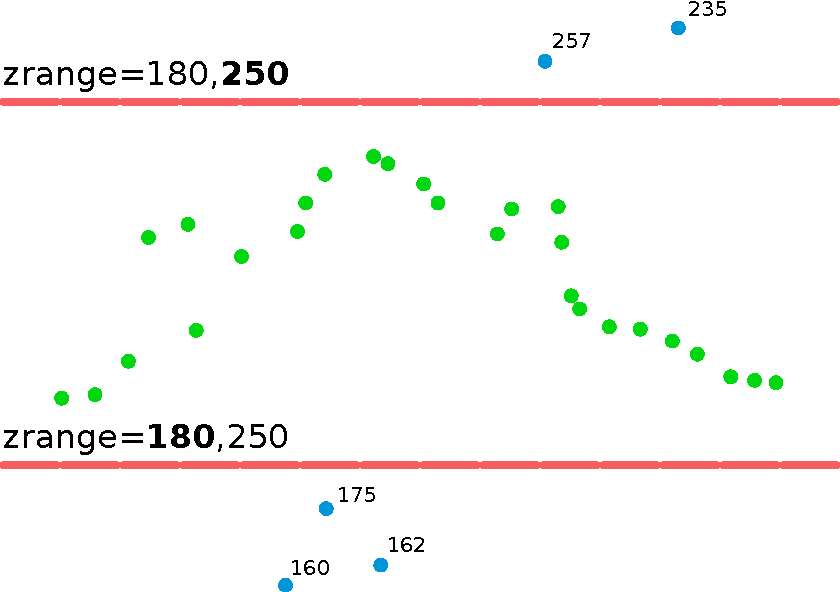
\includegraphics[width=0.88\textwidth]{features/zrange}
\end{center}

\end{column}
\end{columns}

\end{frame}

%%%%%%%%%%%%%%%%%%%%%%%%%%%%%%%%%%%%%%%%%%%%%%%%%%%%%%%%%%%%%%%%%%%%%
\begin{frame}{Height above a surface}
% TODO: diff resolutions

\begin{itemize}
  \item \gmodule{r.in.lidar}, option \textit{base\_raster}
  \item given surface $+$ points cloud
    $\longrightarrow$ height of features
\end{itemize}

\begin{center}
  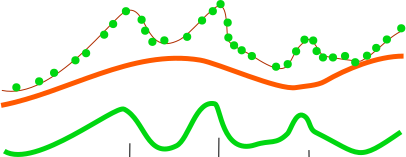
\includegraphics[width=0.7\textwidth]{images/features/base_raster}
\end{center}

\begin{itemize}
  \item low additional memory requirements
\end{itemize}

\end{frame}

%%%%%%%%%%%%%%%%%%%%%%%%%%%%%%%%%%%%%%%%%%%%%%%%%%%%%%%%%%%%%%%%%%%%%
\begin{frame}{Height above a surface}

\begin{columns}
\begin{column}{0.4\textwidth}

\begin{itemize}
 \item different resolutions
  \begin{itemize}
    \item \rule{0pt}{0pt}\phantom{0}1m ground surface
    \item 30m height above ground
  \end{itemize}
  \item different statistics
  \item different combinations
  \begin{itemize}
    \item surface can be e.g. top of the canopy
    \item combine with \textit{zrange}
    \item combine with intensity
  \end{itemize}
\end{itemize}

\end{column}
\begin{column}{0.55\textwidth}

\begin{center}
  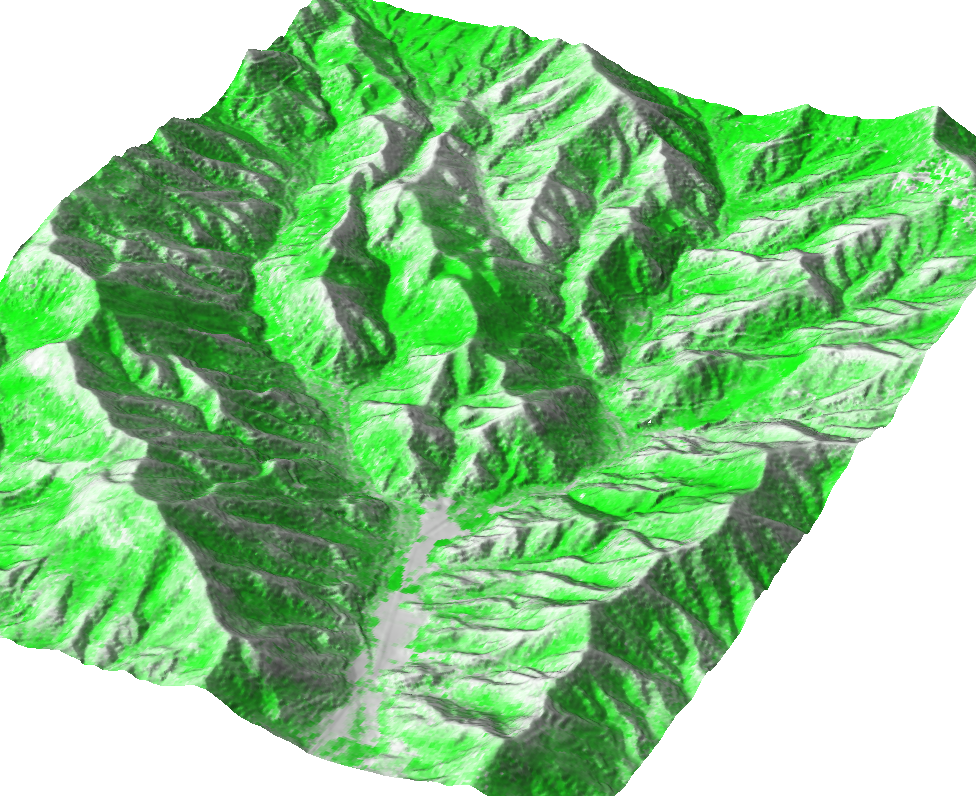
\includegraphics[width=\textwidth]{grass/max_height_10m_on_ground_from_neighbors_smaller_area_top}
\end{center}

\end{column}
\end{columns}

\end{frame}


%%%%%%%%%%%%%%%%%%%%%%%%%%%%%%%%%%%%%%%%%%%%%%%%%%%%%%%%%%%%%%%%%%%%%
\begin{frame}{Rastersize early}

\begin{columns}
\begin{column}{0.5\textwidth}

\begin{itemize}
  \item many algorithms are raster-based
  \begin{itemize}
    \item a lot of data with continuous nature
    \item natural spatial index
  \end{itemize}
  \item example:
  \begin{enumerate}
    \item count of ground points
    \item count of non-ground points
    \item used as image bands
    \item segmentation using \gmodule{i.segment}
  \end{enumerate}
\end{itemize}

\end{column}
\begin{column}{0.45\textwidth}

\begin{center}
  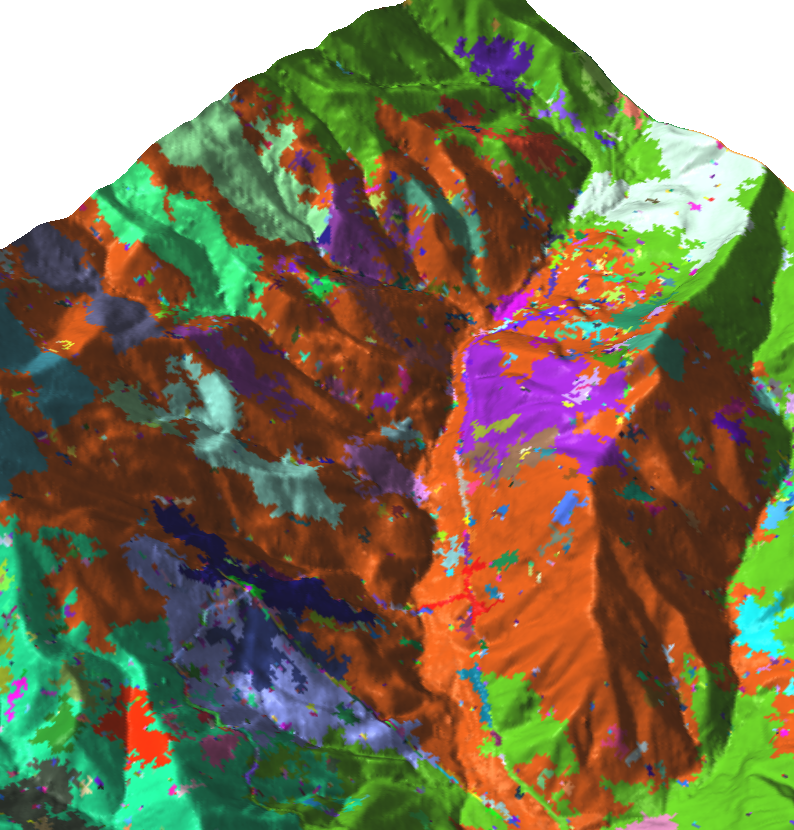
\includegraphics[width=0.9\textwidth]{grass/segment_on_counts}
\end{center}

\end{column}
\end{columns}

\end{frame}

%%%%%%%%%%%%%%%%%%%%%%%%%%%%%%%%%%%%%%%%%%%%%%%%%%%%%%%%%%%%%%%%%%%%%
\begin{frame}{3D raster}

\begin{columns}
\begin{column}{0.38\textwidth}

\begin{itemize}
  \item stacked 2D rasters
  \item challenging to visualize
  \item same principles as in~2D
  \begin{itemize}
  \item e.g. 3D raster map algebra
  \end{itemize}
\end{itemize}

\end{column}
\begin{column}{0.5\textwidth}

\begin{center}
  \includegraphics<1>[width=\textwidth]{grass/raster_3d_cube}
  \includegraphics<2>[width=\textwidth]{grass/raster_3d_slices}
\end{center}

\end{column}
\end{columns}

% vis also possible using Tangible Landscape

\end{frame}


%%%%%%%%%%%%%%%%%%%%%%%%%%%%%%%%%%%%%%%%%%%%%%%%%%%%%%%%%%%%%%%%%%%%%
\begin{frame}{Binning points to 3D raster}

\begin{columns}
\begin{column}{0.28\textwidth}

\begin{itemize}
  \item \gmodule{r3.in.lidar}
  \item proportional count
  \begin{itemize}
    \item count per 3D cell relative to the count per vertical column
  \end{itemize}
  \item intensity can be used instead of count
\end{itemize}

\end{column}
\begin{column}{0.7\textwidth}

\begin{center}
  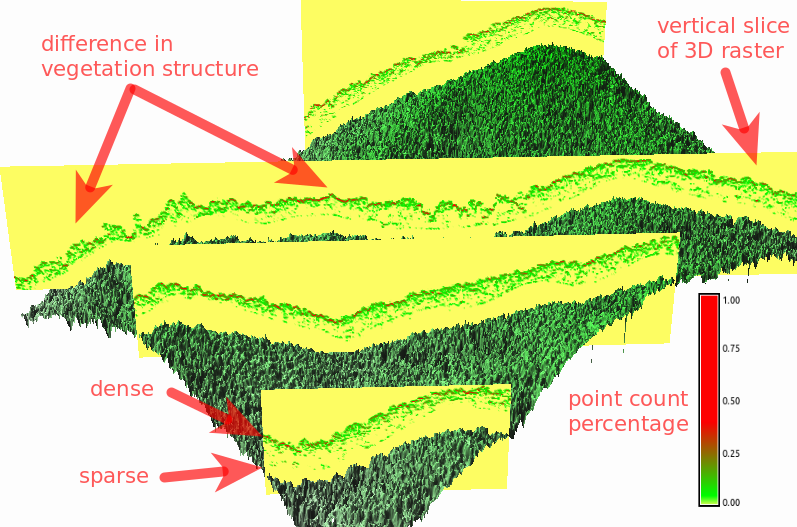
\includegraphics[width=\textwidth]{grass/red_green_3d_labels}
\end{center}

\end{column}
\end{columns}

\end{frame}

%%%%%%%%%%%%%%%%%%%%%%%%%%%%%%%%%%%%%%%%%%%%%%%%%%%%%%%%%%%%%%%%%%%%%
\begin{frame}{Point heights reduced to surface}

\begin{center}
  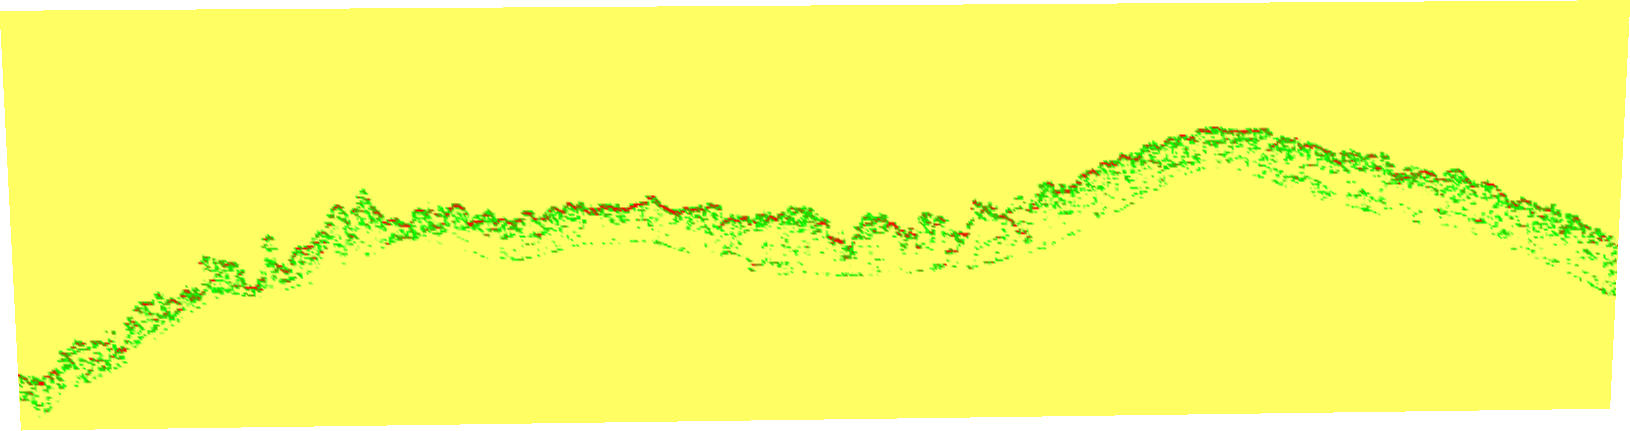
\includegraphics[width=0.8\textwidth]{features/rast3_real}

  \bigskip

  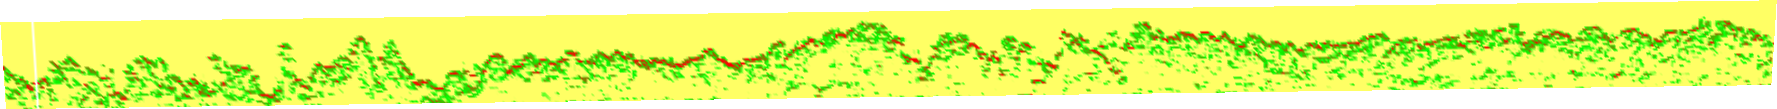
\includegraphics[width=0.8\textwidth]{features/rast3_base}
\end{center}

\begin{itemize}
  \item \gmodule{r3.in.lidar}, option \textit{base\_raster}
  \item height reduced by raster values
\end{itemize}

\end{frame}


%%%%%%%%%%%%%%%%%%%%%%%%%%%%%%%%%%%%%%%%%%%%%%%%%%%%%%%%%%%%%%%%%%%%%
\begin{frame}{Trade-offs}

\begin{columns}
\begin{column}{0.44\textwidth}

Raster processing

\begin{itemize}
  \item hight memory (RAM) usage -- fast
  \item low memory usage (high I/O) -- slow
\end{itemize}

Vector processing

\begin{itemize}
  \item slower than raster
  \begin{itemize}
  \item e.g., interpolation much slowed than binning
  \end{itemize}
  \item hard to make general statements
\end{itemize}

\end{column}
\begin{column}{0.44\textwidth}

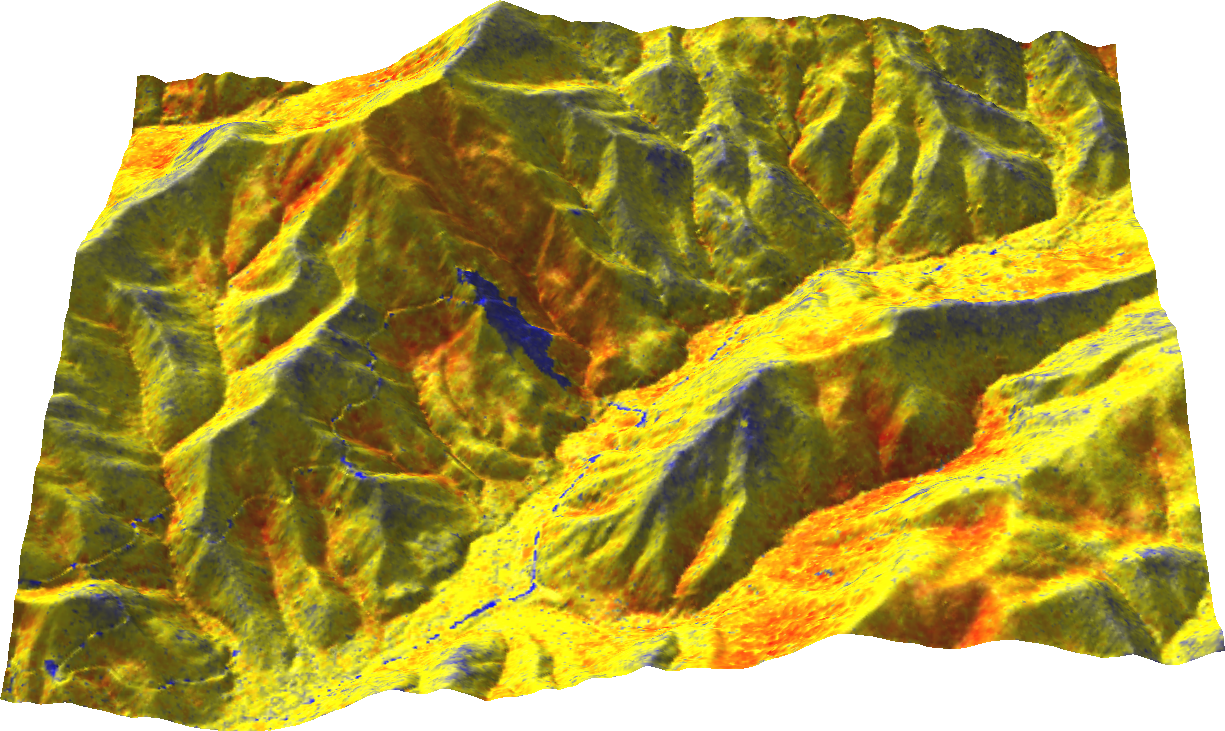
\includegraphics[width=\textwidth]{grass/range_on_ground_from_north}
  \begin{center}
  \tiny
  \textcolor{gray}{
  visualization: range from binning on interpolated surface
  }
  \end{center}

\bigskip

\textcolor{gray}{
\footnotesize
example: binning with base elevation subtraction: $\approx$1000 files, $>9$~billion points
\\
$\approx$3~hours, $\approx$10GB of memory \tiny (in-memory mode)
}

\end{column}
\end{columns}

\end{frame}


%%%%%%%%%%%%%%%%%%%%%%%%%%%%%%%%%%%%%%%%%%%%%%%%%%%%%%%%%%%%%%%%%%%%%
\begin{frame}{Ground detection}

\begin{columns}
\begin{column}{0.35\textwidth}

\begin{itemize}
\item \gmodule{v.lidar.edgedetection}, \gmodule{v.lidar.growing}, \gmodule{v.lidar.correction}
\begin{itemize}
  \item \tiny by Brovelli, Cannata, Antolin \& Moreno
\end{itemize}

\item \amodule{v.lidar.mcc}
\begin{itemize}
  \item \tiny multiscale curvature based classification algorithm
  \item \tiny by Blumentrath, according to Evans \& Hudak
\end{itemize}

\item PDAL filters.ground
\begin{itemize}
  \item \tiny now in v.in.pdal
  \item \tiny progressive morphological filter by Zhang
  \item \tiny provided by PCL
\end{itemize}

\end{itemize}

\end{column}
\begin{column}{0.64\textwidth}

\begin{center}
  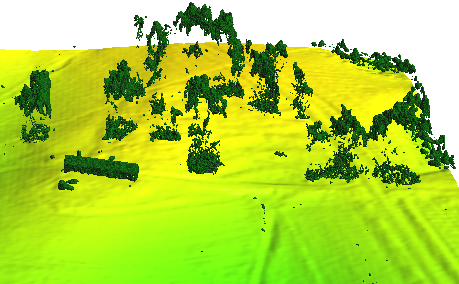
\includegraphics[width=\textwidth]{grass/mcc_default_smaller}
\end{center}

\end{column}
\end{columns}

\end{frame}


%%%%%%%%%%%%%%%%%%%%%%%%%%%%%%%%%%%%%%%%%%%%%%%%%%%%%%%%%%%%%%%%%%%%%
\begin{frame}{Sky-view factor}

\begin{itemize}
  \item \amodule{r.skyview} (percentage of visible sky)
\end{itemize}

\begin{center}
  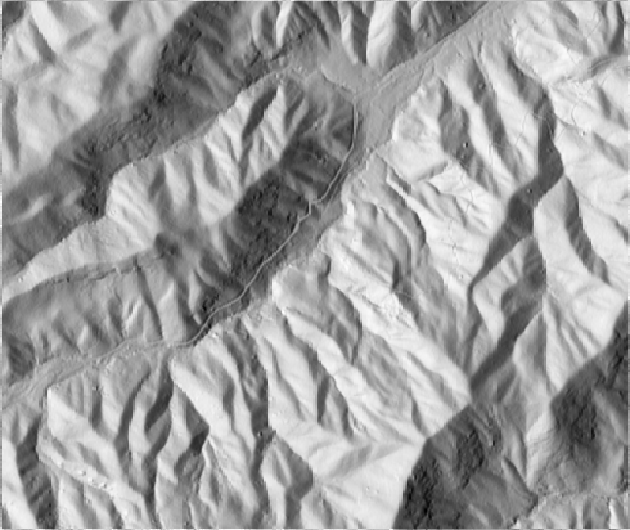
\includegraphics[width=0.45\textwidth]{vis/shade}
  ~
  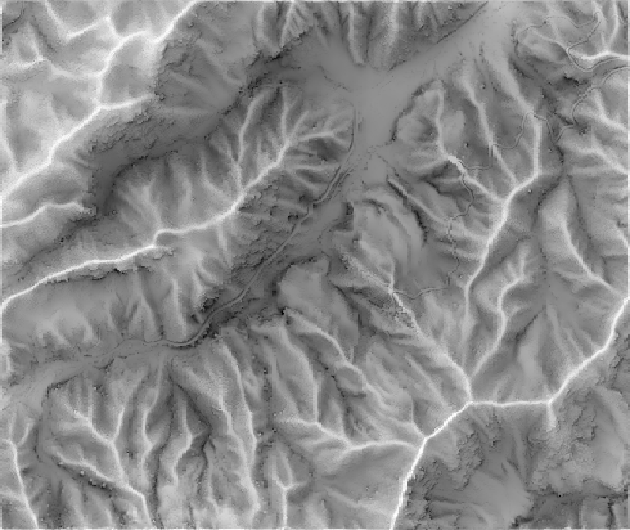
\includegraphics[width=0.45\textwidth]{vis/skyview_ridges}
  \\
  {\footnotesize comparison of shaded relief and sky-view factor}
  % 412*4 (1648) x 490*4 (1960)
\end{center}

\end{frame}


%%%%%%%%%%%%%%%%%%%%%%%%%%%%%%%%%%%%%%%%%%%%%%%%%%%%%%%%%%%%%%%%%%%%%
\begin{frame}{Local relief model (LRM)}

\begin{itemize}
  \item \amodule{r.local.relief} (micro-topography, features other than trend)
\end{itemize}

\begin{center}
  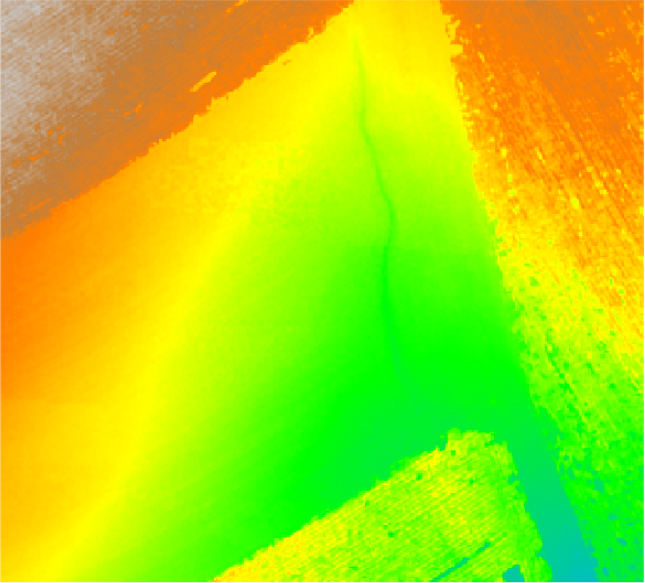
\includegraphics[width=0.4\textwidth]{vis/elevation}
  ~~
  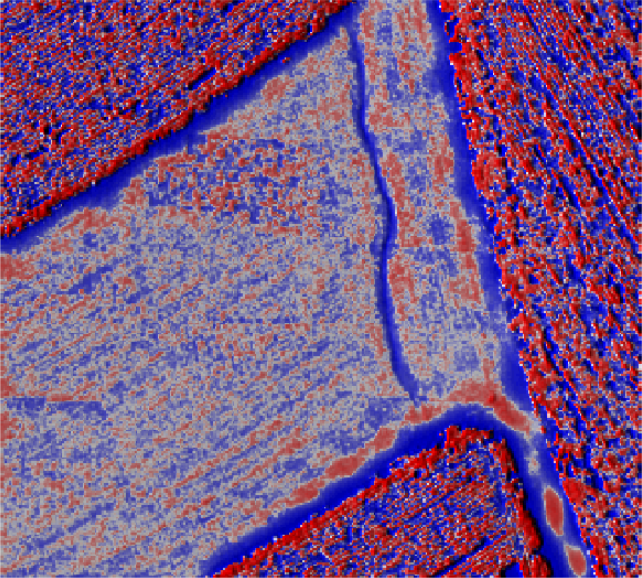
\includegraphics[width=0.4\textwidth]{vis/lrm}\\
  \footnotesize
  30-60cm wide, 30cm deep, 60m long gully (resolution 30cm)
  % 294 rows, 325 cols (88.2m x 97.5m)
\end{center}

\end{frame}


%%%%%%%%%%%%%%%%%%%%%%%%%%%%%%%%%%%%%%%%%%%%%%%%%%%%%%%%%%%%%%%%%%%%%
\begin{frame}{Landforms}

\begin{columns}
\begin{column}{0.3\textwidth}

\begin{itemize}
  \item \amodule{r.geomorphon}
  \begin{itemize}
  \item new landform classification approach
  \item by Jasiewicz \& Stepinski
  \end{itemize}
\end{itemize}

\end{column}
\begin{column}{0.68\textwidth}

\begin{center}
  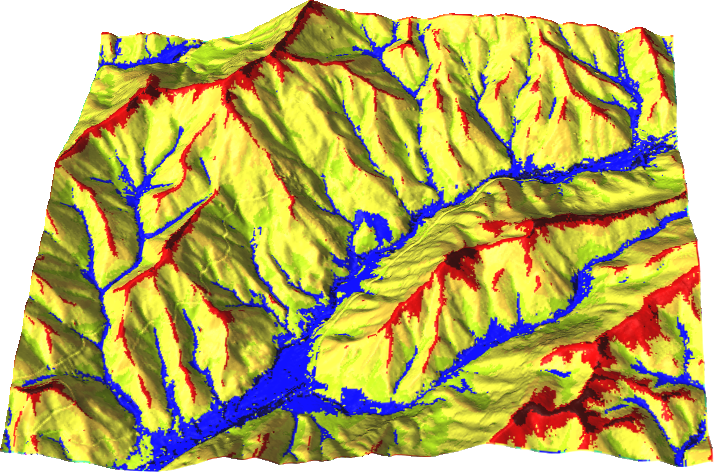
\includegraphics[width=\textwidth]{vis/geomorphon_3d}
\end{center}

\end{column}
\end{columns}

\end{frame}


%%%%%%%%%%%%%%%%%%%%%%%%%%%%%%%%%%%%%%%%%%%%%%%%%%%%%%%%%%%%%%%%%%%%%
\begin{frame}{libfreenect2 + PCL + GRASS GIS = \module{r.in.kinect}}

\begin{columns}
\begin{column}{0.5\textwidth}

\begin{block}{\module{r.in.kinect}}
 \begin{itemize}
  \item scans using Kinect
  \item OpenKinect libfreenect2
  \item Point Cloud Library (PCL)
  \item GRASS GIS libraries
  \begin{itemize}
    \item C API
    \item raster processing
    \item regularized spline with tension interpolation
  \end{itemize}
 \end{itemize}
\end{block}

% inner columns
\begin{columns}
\begin{column}{0.6\textwidth}
\small

used in Tangible~Landscape

\end{column}
\begin{column}{0.2\textwidth}

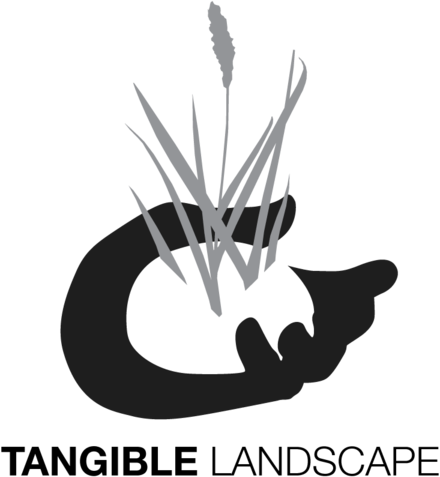
\includegraphics[width=\textwidth]{logos/tangible_landscape}

\end{column}
\end{columns}
% end of inner columns

\end{column}
\begin{column}{0.45\textwidth}

\begin{center}
  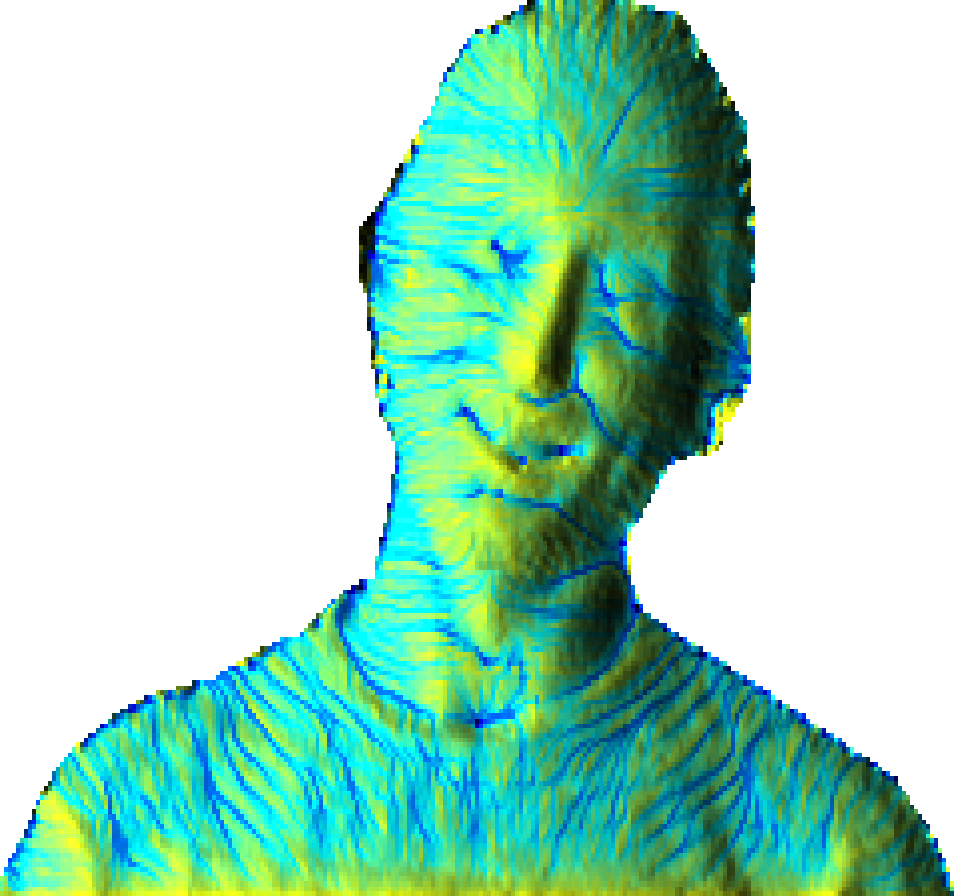
\includegraphics[width=\textwidth]{tangible/face}
\end{center}

\end{column}
\end{columns}

\end{frame}



%%%%%%%%%%%%%%%%%%%%%%%%%%%%%%%%%%%%%%%%%%%%%%%%%%%%%%%%%%%%%%%%%%%%%
\begin{frame}{}

% logo at the bottom can be moved down
\vspace*{0.05\textheight}

\begin{block}{Summary}
 \begin{itemize}
  \item rasterize early
  \item make use of existing methods for raster and vector processing
  \item 3D rasters, PDAL integration
 \end{itemize}
\end{block}

\bigskip
\centering

\begin{tabular}{clc}
\begin{minipage}{0.16\textwidth}

\includegraphics[width=\textwidth]{logos/grass_gis}
\end{minipage}
&
\begin{minipage}{0.5\textwidth}
\footnotesize
\href{https://grass.osgeo.org/download/}{%
Get GRASS GIS 7.1 development version at\\
\texttt{grass.osgeo.org/download}%
}

\bigskip

{
\footnotesize
Slides and paper available at\\
\href{http://wenzeslaus.github.io/grass-lidar-talks/}%
  {\texttt{wenzeslaus.github.io/grass-lidar-talks}}
}

{
\footnotesize
\href{https://lists.osgeo.org/listinfo/grass-user}{GRASS user mailing list}\\
\href{https://lists.osgeo.org/listinfo/grass-user}{\texttt{lists.osgeo.org/listinfo/grass-user}}
}
\end{minipage}
&
\begin{minipage}{0.2\textwidth}

\includegraphics[width=\textwidth]{talks_qr}
\end{minipage}
\end{tabular}

\end{frame}

% don't count the backup and ack slides
\backupbegin

%%%%%%%%%%%%%%%%%%%%%%%%%%%%%%%%%%%%%%%%%%%%%%%%%%%%%%%%%%%%%%%%%%%%%
\begin{frame}{Acknowledgements}

\begin{columns}
\begin{column}{0.6\textwidth}

\begin{block}{Software}
Presented functionality is work done by Vaclav Petras, Markus Metz, and the GRASS development team.

\bigskip

Thanks to users for feedback and testing, especially to
Doug Newcomb, Helena Mitasova, Markus Neteler, Laura Belica, and William Hargrove.
\end{block}

\end{column}
\begin{column}{0.3\textwidth}

\begin{center}
  
\includegraphics[width=\textwidth]{logos/grass_gis}
\end{center}

\end{column}
\end{columns}

\end{frame}


%%%%%%%%%%%%%%%%%%%%%%%%%%%%%%%%%%%%%%%%%%%%%%%%%%%%%%%%%%%%%%%%%%%%%
\begin{frame}{Acknowledgements}

\begin{columns}
\begin{column}{0.48\textwidth}

\begin{block}{Datasets}
\footnotesize
Lidar and UAV Structure from Motion (SfM) data for
\href{http://ncsu-osgeorel.github.io/uav-lidar-analytics-course/}%
  {GIS595/MEA792: UAV/lidar Data Analytics} course

\smallskip

Nantahala NF, NC: Forest Leaf Structure, Terrain and Hydrophysiology.
% Lidar data acquisition and processing completed
% by the National Center for Airborne Laser Mapping (\href{http://www.ncalm.org}{NCALM}).
% NCALM funding provided by NSF's Division of Earth Sciences, Instrumentation and Facilities Program.
% EAR-1043051.
Obtained from \href{http://www.opentopography.org/}{OpenTopography}.
\url{http://dx.doi.org/10.5069/G9HT2M76}
\end{block}

\end{column}
\begin{column}{0.47\textwidth}

\begin{center}
  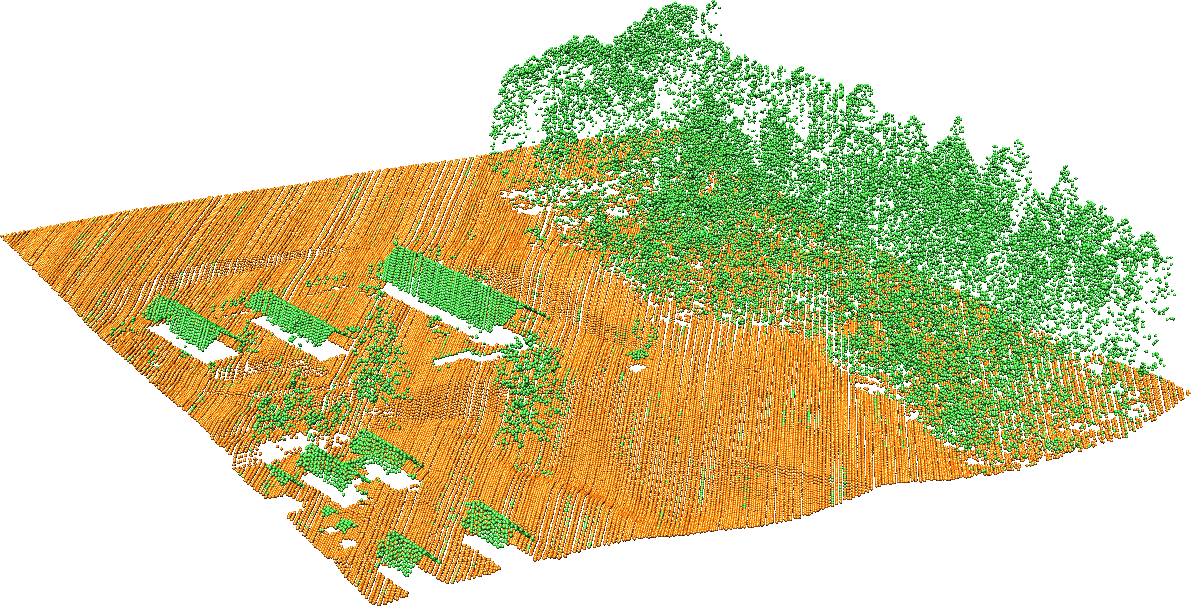
\includegraphics[width=\textwidth]{lidar_secref_3d}
\end{center}

\end{column}
\end{columns}

\end{frame}

%%%%%%%%%%%%%%%%%%%%%%%%%%%%%%%%%%%%%%%%%%%%%%%%%%%%%%%%%%%%%%%%%%%%%
\begin{frame}{Acknowledgements}

\begin{block}{Presentation software}
\Huge
\textrm{Slides were created in \LaTeX{} using the~\textsc{beamer} \textit{class}.}
% all lowercase, sc and it taken from the beamer user guide
\end{block}

\end{frame}

\backupend

\end{document}
